%\documentclass[onecolumn, 12pt]{book}
%
%\usepackage[latin1]{inputenc}   
%\usepackage{amsmath}
%\usepackage{algorithm}
%\usepackage{algorithmic} 
%%\usepackage[T1]{fontenc}
%
%%\usepackage[francais]{babel}     
%\usepackage{layout}    
%\usepackage[top=2cm, bottom=2cm, left=2cm, right=2cm]{geometry} 
%\usepackage{setspace}
%\usepackage{soul}
%\usepackage{color} 
%\usepackage{verbatim}
%\usepackage{moreverb}
%\usepackage{listings}
%\usepackage{url}
%\usepackage{graphicx}
%\usepackage{epstopdf}
%\usepackage{caption}
%\usepackage{setspace}
% \usepackage{amssymb} % used for not exists symbol ==> \nexists
% 
%\title{algorithme de correction}
%\author{Wilfried Ehounou}
%\date{\oldstylenums{\today}} 
%
%\newtheorem{definition}{D\'efinition}
%\newtheorem{property}{Propri\'et\'e}
%\newtheorem{theorem}{Theorem}
%\newtheorem{claim}[theorem]{Claim}
%\newtheorem{proposition}[theorem]{Proposition}
%\newtheorem{lemma}[theorem]{Lemma}
%\newtheorem{corollary}[theorem]{Corollary}
%\newtheorem{conjecture}[theorem]{Conjecture}
%\newtheorem{observation}{Observation}
%\newtheorem{example}{Exemple}
%\newtheorem{remark}{Remark}
%
%%---insert paragraph (use 4) and subparagraph (use 5) to table of contents
%\setcounter{tocdepth}{4} 
%\setcounter{secnumdepth}{4}
%
%%---- path figures ----
%\graphicspath{{/home/willy/Documents/courbePython/courbeDegreCoutMinAleatoire_11_09_2017/}
%{/home/willy/Documents/courbePython/courbeDegreCoutMinAleatoire_11_10_2017/}
%{/home/willy/Documents/courbePython/courbeDegreCoutMinAleatoire_11_09_2017/comparaison_MethodesCorrection_fctDeCout_permut_aleatoire_coutMin_degreMin/}{/home/willy/Documents/latexDoc/redactionThese/chap3_linegraphs/imagesLineGraphes/}}
% 
%\begin{document}
%\maketitle
%\tableofcontents

\section{Correction de la matrice de corr\'elation}
Si le graphe $G_C=(V_C, E_C)$ est un graphe de corr\'elation alors l'algorithme de couverture determine sa line couverture $\cal C$.
En effet, par r\'ecurrence sur l'ensemble des sommets, on montre \`a chaque \'etape qu'il existe un sommet non encore couvert qui soit :
\begin{itemize}
\item  est couvert par une clique appartenant \`a $\cal C$ et son voisinage restant et lui peuvent \^etre converts par une nouvelle clique.
\item n'est couvert par aucune clique de  $\cal C$ et son voisinage restant et lui peuvent \^etre couverts par une ou deux nouvelles cliques.
\end{itemize}
Dans le cas o\`u la line-couverture de $G_C$ ne peut \^etre fournie \`a cause des erreurs de corr\'elations, nous avons des sommets couverts par soit aucune clique ou soit par plus de deux cliques. Ces sommets, labellis\'es \`a $-1$, forment l'ensemble 
$sommets\_1 = \{\exists z \in V, Cliq(z) = -1 \}$ 
et sont appel\'es {\em sommets \`a corriger}.
\newline

Nous proposons l'{\em algorithme de correction} qui va modifier l'ensemble initial $E_C$ par ajout et suppression d'ar\^etes dans le but d'obtenir un {\em line graphe}.
Nous allons consid\'erer un ordre $O_z = [z_1, z_2, \cdots, z_t]$ de sommets de $sommets\_1$ qui correspond au mode de s\'election de ceux-ci pendant la phase de correction.
Il en suit que l'ordre a une influence sur le line graphe fourni parce que la correction modifie le voisinage des sommets. Il est montr\'e dans la chapitre \ref{simulationsTheoriques}.
\newline
Soit $E_C^i$ l'ensemble des ar\^etes de $G_C$ apr\`es le traitement des $i-1$ premiers sommets dans l'ordre $O_z$. De m\^eme, on note ${\cal C}^i$ l'ensemble des cliques de $G_C$ \`a l'\'etape $i$ et donc $E_C^1 = E_C$ et ${\cal C} = {\cal C}^1$.
\newline

Soient $z=z_i$ le i-i\`eme sommet et ${\cal C}(z) = \{C_1, \cdots, C_k\}$ l'ensemble des cliques de ${\cal C}^i$ de taille sup\'erieure ou \'egale \`a $3$ auxquelles le sommet $z$ appartient.
Notons que, par d\'efinition et par construction, chaque paire de cliques dans ${\cal C}(z)$ n'a que $z$ comme sommet commun et que $S(z)$ est l'union des voisins $v$ de $z$ dans des cliques $\{v,z\} \in {\cal C}^i$ de taille $2$ et des voisins $v$ de $z$ tels que l'ar\^ete $[z,v]$ n'est couverte par aucune clique de ${\cal C}^i$.
\begin{equation}
C(z) = \{C_i, i \in [1,k] \mid  |C_i| \ge 3 \mbox{ } \&  \mbox{ } C_i \in {\cal C}^i \} 
\end{equation}
\begin{equation}
S(z) = \{v \in \Gamma_G(z) \mid \{v,z\} \in {\cal C}^i\} \cup  \{ v \in \Gamma_G(z) \mid \nexists C \in {\cal C}^{i} , [z,v] \in E_C(C) \}
\end{equation}

\begin{definition}
Deux cliques $C$ et $C'$ de ${\cal C}(z)$ sont {\em contractables} si aucune ar\^ete $[u,v]$ de $E_C^i$ telle que $u \in C$ et $v \in C'$ n'est couverte par une clique (autre que ${u,v}$) dans $\cal C$.
Un ensemble de cliques de $\cal C$ est contractable si tous les cliques sont deux \`a deux contractables.
\end{definition}

\begin{definition}
Une clique $C \in C_i$ est {\em voisine} de $z$ si $C \notin {\cal C}(z)$ et $card(C \cap S(z)) \ge 2$.
La d\'ependance d'une clique $C$ voisine de $z$ est l'ensemble $D_z(C) \subset {\cal C}(z)$ tel que $C' \in D_z(C)$ si et seulement si  $C' \cap C \cap \Gamma_{G}(z) \ne \emptyset$.
\newline
Une clique $C$ est {\em augmentante} pour le sommet $z$ si et seulement si elle est voisine de $z$ et  $D_z(C)$ est vide  ou $D_{z}(C) \cup \{C\}$ est contractable.
\begin{equation}
voisine(z) = \{C \in {\cal C}^i \mbox{ } \mid \mbox{ } C \notin C(z) \mbox{ } \& \mbox{ } card(C \cap S(z)) \ge 2 \} \newline
\end{equation}
\begin{equation}
D_{z}(C) = \{ C' \in C(z) \mbox{ } \mid  \mbox{ } C' \cap C \cap \Gamma_{G}(z) \ne \emptyset \}
\end{equation}
\end{definition}

On appelle {\em  augmentation} du sommet $z$ l'union d'une clique augmentante  $C$ pour $z$ et d'une constraction de cliques de $D_z(C)$.

Un exemple de clique augmentante $C1$ pour le sommet $z$ est donn\'e dans la figure \ref{exempleAlgoCorrectionGraphe}, avec $D_z(C1) = \{C2\}$.
Par contre, la clique C6 ne peut pas \^etre augmentante \`a cause de l'appartenance de l'ar\^ete $[u,v]$ \`a la clique $C7$ de $C^i$. Ce qui rend impossible toute contraction entre $C6$ et $C4$
\begin{centering} 
\begin{figure}[htb!]
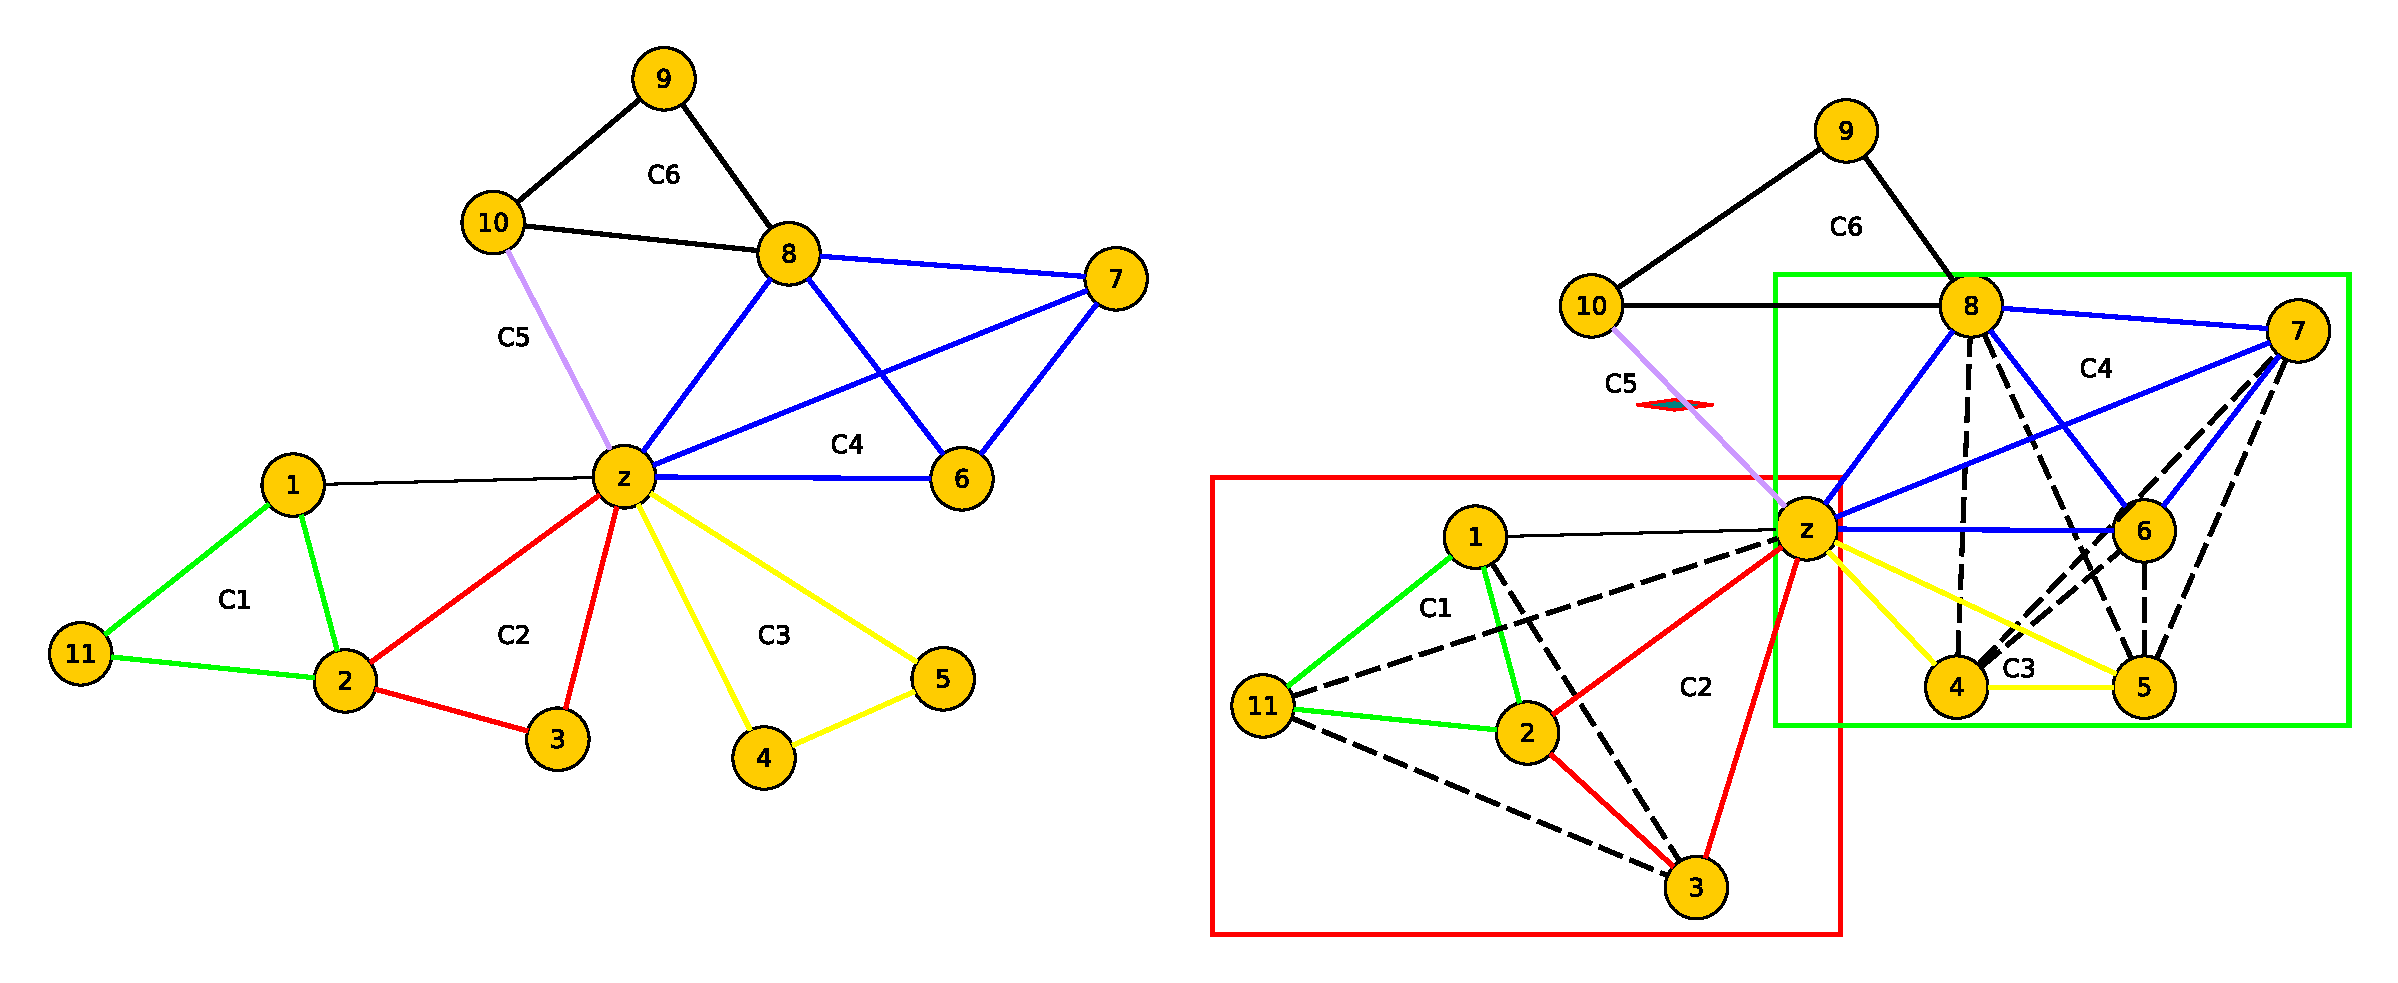
\includegraphics[scale=0.450]{./correctionGraph.eps} \vspace{-0.5em}
\caption{un exemple de compression de cliques}
\label{exempleAlgoCorrectionGraphe}
\end{figure}
\end{centering} 

\begin{definition}
On appelle {\em compression} du sommet $z$ un triplet ($\pi_1$, $\pi_2$ et $\pi_s$) d\'efini par : 
\begin{itemize}
	\item $\pi_1$ (resp. $\pi_2$) peut \^etre  chacun d'une des formes suivantes :
	\begin{enumerate}
		\item l'union de $z$, d'un sous-ensemble $C_1$ (resp. $C_2$) de cliques de ${\cal C}(z)$ tel que toute paire $C$ et $C'$ de $C_1$ (resp. $C_2$) est contractable et d'un sous-ensemble $S_1$ (resp. $S_2$) de sommets $v \in S(z)$ n'appartenant \`a aucune clique de $C_1$ (resp. $C_2$) tel que
		$$ \forall v \in S_1,~\forall x \in C_1, \not\exists C' \in {\cal C}~t.q.~card(C')>2~~et~~\{v,x\} \subset C'$$
		(ce qui fait que \{v,x\} peut etre une clique de ${\cal C}^i$).
		\item une augmentation du sommet $z$
	\end{enumerate}
	\item $\pi_1$ et $\pi_2$ ne peuvent pas \^etre simultan\'ement r\'eduits \`a $\{z\}$ et $\pi_1 \cap \pi_2 = \{z\}$,
	\item $\pi_S=\Gamma_G(z)-~((\pi_1 \cap \Gamma_G(z)) \cup(\pi_2 \cap \Gamma_G(z)))$ tel que l'ensemble des ar\^etes  $\{[z,v]\in E_{C}^{i}:~v\in \pi_S\}$ n'est pas d\'econnectant.
	\item le triplet $\pi_{1} \cap \Gamma_{G}(z)$, $\pi_{2} \cap \Gamma_{G}(z)$, $\pi_{S} \cap \Gamma_{G}(z)$  est une 3-partition de $\Gamma_G(z)$
\end{itemize}
\end{definition}
Il existe toujours une telle compression, ne serait-ce que 
$\pi_1 = \{z\} \cup C_i \in C(z)$, 
$\pi_2 =  \emptyset$,
$\pi_s = \gamma_G(z) -(\gamma_G(z) \cup C_i) $  si ${\cal C}(z)$ n'est pas vide.
Sinon, 
$\pi_1 = \{z\} \cup \{ v \in \gamma_G(z)  \} $, 
$\pi_2 =  \emptyset$,
$\pi_s = \gamma_G(z) - \{v\} $
est aussi une compression.
Un exemple de compression est aussi donn\'e dans la figure \ref{exempleAlgoCorrectionGraphe}.
Le co\^ut $c(T)$ d'une compression $\pi_{1},\pi_{2},\pi_{S}$ est d\'efini par : 
$$c(T) = | \{\{u,v\} \in \pi_{1}:~[u,v]\not\in E_{C}^{i}\}| + |\{\{u,v\} \in \pi_2:~[u,v]\not\in E_{C}^{i}\}| +~ |\pi_S| $$
Dans l'exemple de la figure \ref{exempleAlgoCorrectionGraphe}(a), autour d'un sommet $z$, l'ensemble $C(z)$ contient les cliques $C2$, $C3$,$C4$ et $C5$.
Les cliques $C5$ et $C4$ ne sont pas contractables, \`a cause de l'existence de $C6$ dans ${\cal C}_i$.
La clique $C1$ est voisine de $z$ et $D(C1) = \{C2\}$.
L'exemple de compression qui est donn\'e dans la figure \ref{exempleAlgoCorrectionGraphe}(b) est $\pi_1 = C1 \cup C2$ (une augmentation), $\pi_2 = C3 \cup C4$ (ces deux cliques \'etant contractables), et $\pi_s = \{x\}$.
Le co\^ut  de cette compression est $10$, $10$ \'etant le nombre d'ar\^etes en pointill\'e plus l'ar\^ete supprim\'ee $[x,z]$.
\newline

Soit  $Cout(z)$ le co\^ut minimum d'une compression de $z$.
Le but est de modifier $G_C$ afin que $z$ puisse \^etre couvert par une ou deux cliques issues de $\pi_1$ et $\pi_2$.
Pour cela, le co\^ut de cette modification $c(T)$ tient compte des ar\^etes \`a ajouter (li\'ees \`a $\pi_1$ et $\pi_2$) et \`a supprimer (li\'ees \`a $\pi_s$).
\newline
Ainsi, {\bf appliquer une compression} $T = \pi_1, \pi_2, \pi_s$ consiste \`a ajouter dans $E_C^i$ les ar\^etes d\'efinies par les ensembles de paires $\{\{u,v\} \in \pi_1:~[u,v]\not\in E_{C}^{i}\}$ (qui seront couvertes par la clique $\pi_1$) et $\{\{u,v\} \in \pi_2:~[u,v]\not\in  E_{C}^{i}\}$ (qui seront couvertes par la clique $\pi_2$) et \`a supprimer les ar\^etes $\{[z,v] \in  E_{C}^{i}:~v\in \pi_S\}$. 
\newline
Des lors, le sommet $z$ appartient aux deux cliques $\pi_1$ et $\pi_2$.
On proc\`ede alors aux mises \`a jour suivantes pour obtenir ${\cal C}^{i+1}$ et $E_C^{i+1}$ :
\begin{itemize}
\item supprimer toutes les cliques ${\cal C}_z$ couvertes par $\pi_1$ dans  ${\cal C}^{i}$.
\item supprimer toutes les cliques ${\cal C}_z$ couvertes par $\pi_2$ dans  ${\cal C}^{i}$.
\item supprimer toutes les cliques de cardinalit\'e $2$ couvertes par $\pi_1$ et $\pi_2$ dans  ${\cal C}^{i}$.
\item ajouter $\pi_1$ et $\pi_2$ dans ${\cal C}^{i}$, supprimer de $E_C^{i+1}$ toutes les ar\^etes  $\{[z,v] \in E_C^{i}:~v\in \pi_S\}$.
\item Affecter $Cliq(z)$ \`a $1$ (si $\pi_1$  ou $\pi_2$ est vide) ou $2$ (sinon).
\end{itemize}
Cette proc\'edure a les propri\'et\'es suivantes :
\begin{property}
Consid\'erons une application d'une compression,
Soit ${\cal C}^{i+1}$  l'ensemble obtenu \`a partir de ${\cal C}^{i}$ apr\`es  mise \`a jour selon cette application.
\begin{itemize}
	\item Tout sommet de $G_C$ couvert par une ou deux cliques dans ${\cal C}^{i}$ le reste dans ${\cal C}^{i+1}$.
	\item Toute ar\^ete couverte par une et une seule clique dans ${\cal C}^{i}$ et qui n'est pas supprim\'ee le reste dans ${\cal C}^{i+1}$.
	\item Le sommet $z$ est couvert par une ou deux cliques dans ${\cal C}^{i+1}$ (le nombre de sommets ainsi couverts augmente de $1$ par rapport \`a celui dans ${\cal C}^{i}$).
\end{itemize}
\end{property}

Ainsi, pour chaque sommet $z_i$ pris dans l'ordre $O_z$, on consid\`ere une compression de co\^ut minimum $c_m^i$ et on l'applique.
La propri\'et\'e ci-dessus garantit qu'\`a l afin du processus, on obtientun graphe de corr\'elation $G_C^t = (V, E_C^t)$ dont l'ensemble $\cal C$ modifi\'e est une couverture de corr\'elation. 
La distance-line v\'erifie  
$$DL( G_{C}^{0}, G_{C}^{t}) \le \sum_{1 \le i \le t } c_{m}^{i}$$
Notons que lors d'une \'etape $j > 1$, le sommet $z_j$ et son voisinage se retrouve \^etre couvert par une ou deux cliques suite au traitement des $j-1$ sommets pr\'ec\'edents, aucune compression ne lui est appliqu\'ee (on consid\`ere la compression identit\'e) et donc 
$c_{m}^{i} = 0$.



%\end{document}